\documentclass{sciposter}
\usepackage{lipsum}
\usepackage{epsfig}
\usepackage{amsmath}
\usepackage{amssymb}
\usepackage{multicol}
\usepackage{graphicx,url}
\usepackage{textpos}   
\usepackage[utf8]{inputenc}
\usepackage{xcolor}
\usepackage{tabularx}
\newtheorem{Def}{Definition}

% project title
\title{
	\leavevmode{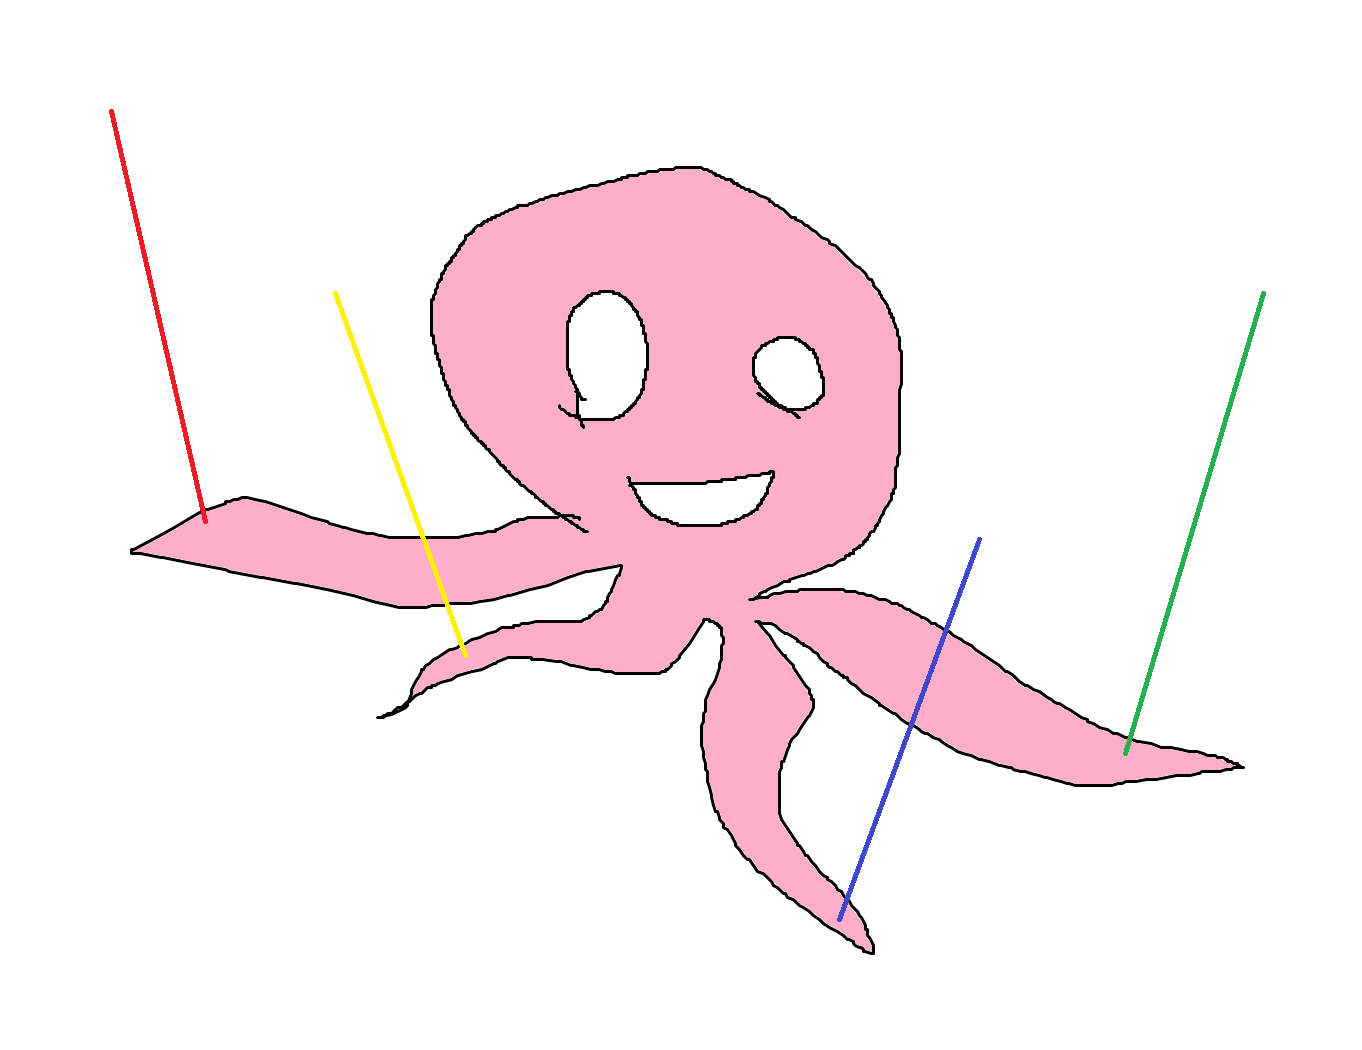
\includegraphics[width=0.3\textwidth]{../Logos/gestikulaser.png}}\\
	Gestikulaser
}

% authors
\author{Christoph Behr, Cailing Fu, Nicole Grubert, Daniel Wolff}

%\renewcommand\printleftlogo
%  {\begin{center}
%     \resizebox{\textwidth}{!}%
%       {
\includegraphics{TOSLogo.png}
\includegraphics{COSIMALogo.png}}
%   \end{center}
%  }
  
%\rightlogo[2]{TOSLogo.png}
%\leftlogo[2]{COSIMALogo}

% Section title color:
\definecolor{SectionCol}{rgb}{0.0, 0.329411, 0.62353} % RWTH Blau
% Section block color:
\definecolor{BoxCol}{rgb}{0.949,0.949,0.949} % Grau

\begin{document}

% TOS Logo oben links
\begin{textblock*}{60px}(0cm,0cm)
	
\includegraphics[height=4cm]{../Logos/TOS.png}
\end{textblock*}

% COSIMA18 Logo oben rechts
\begin{textblock*}{60px}(55cm,0mm)
	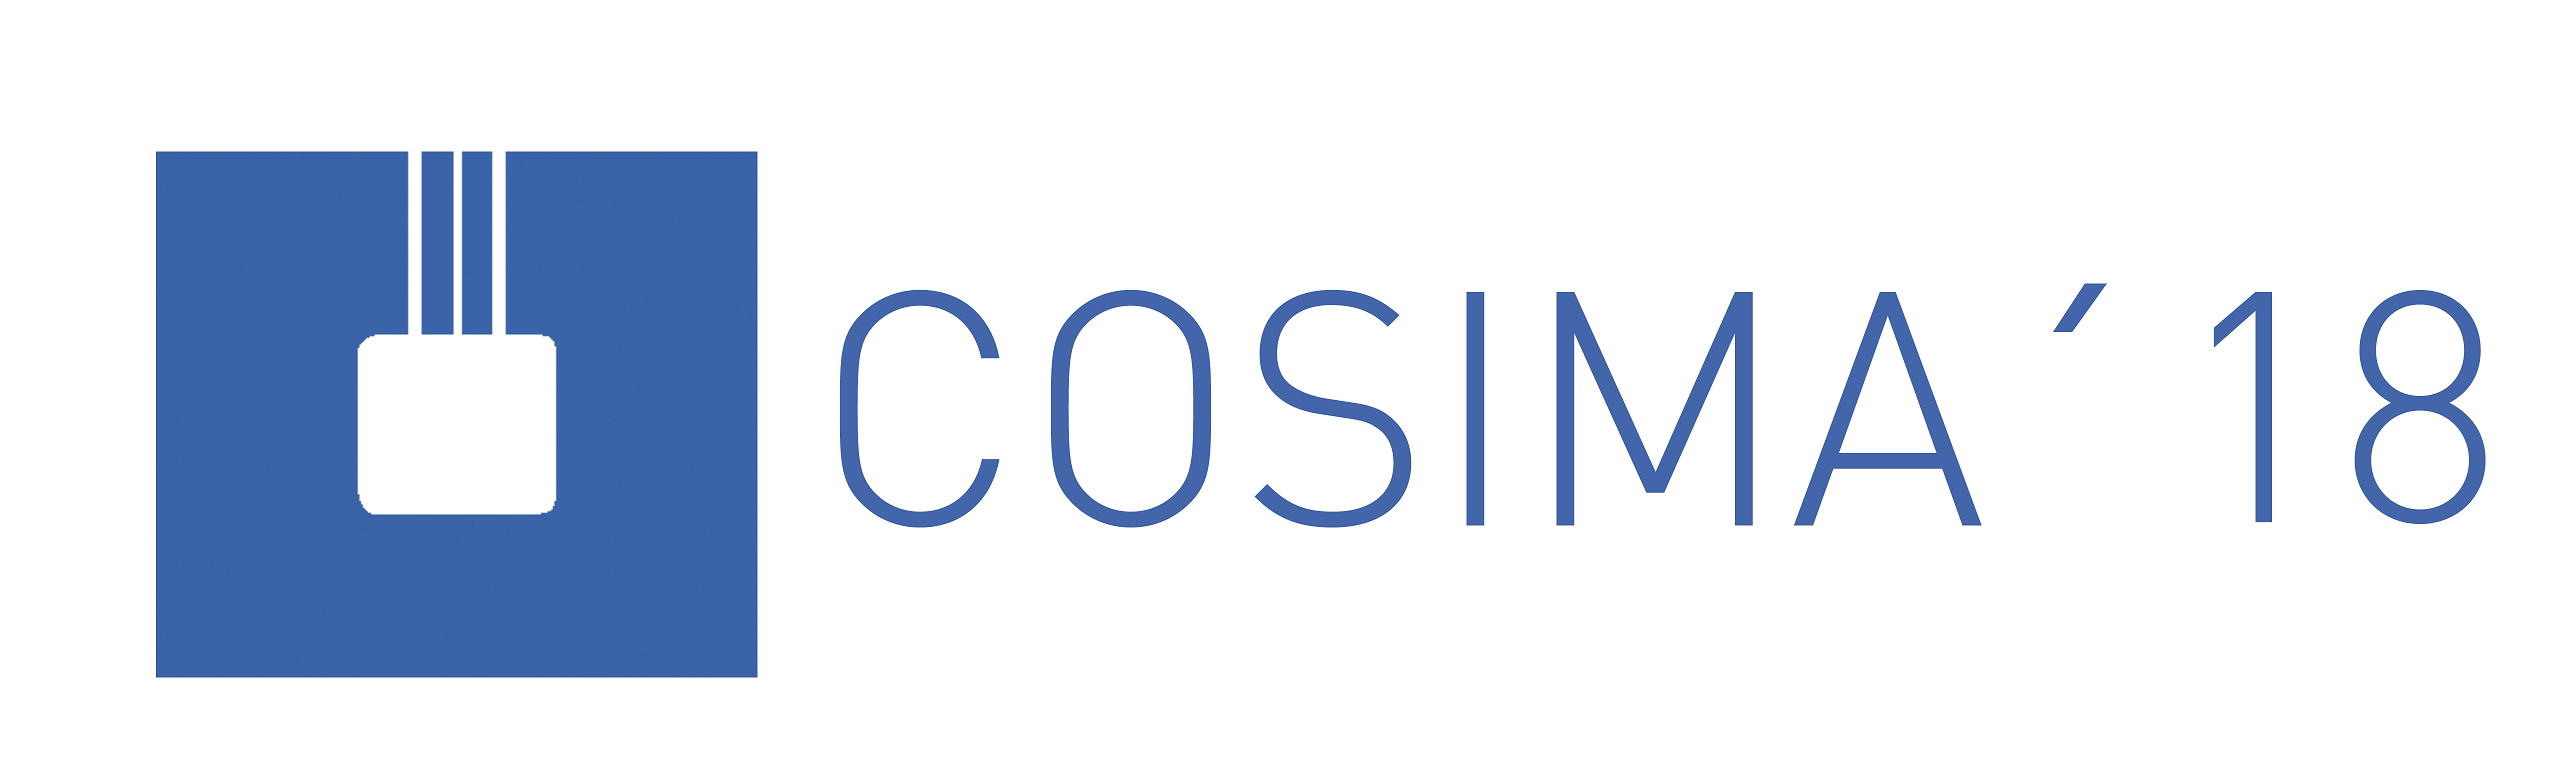
\includegraphics[height=4cm]{../Logos/Cosima18.png}
\end{textblock*}

\maketitle

%%% Begin of Multicols-Enviroment
\begin{multicols}{3}
\setlength{\parindent}{2em}

\section{Unsere Vision}
Gestenerkennung ist immer wieder ein Thema, welches viel Aufmerksamkeit erregt. Und obwohl ein Mensch recht einfach verschiedene Gesten erkennen kann, ist es für den Computer eine große Herausforderung, zuverlässig die Gesten eines Menschen zu erkennen. \\
Mit dem Gestikulaser wollen wir ein neues System entwickeln, um Handgesten eines Menschen zu erkennen. Dabei soll dieses nicht mit einer Kamera arbeiten, wie die meisten heute verfügbaren Systeme, sondern die Hand des Nutzers soll mit Infrarot-LEDs beleuchtet werden und die Gesten sollen durch die erzeugten Reflektionsmuster erkannt werden. Eine auf diese Weise realisierte Gestenerkennung ist nicht nur Tageslicht unabhängig, sondern kann auch in vollkommener Dunkelheit betrieben werden. \\

\section{Der Gestikulaser}
Der Gestikulaser besteht aus zwei Komponenten, einer Photoplatte, sowie einer Machine Learning Software. \\
Die Photoplatte ist mit mehreren infrarot LED Quellen, sowie einer Vielzahl von Photodioden ausgestattet, welche ausschließlich infrarotes Licht detektieren. Durch die Lichtreflexion der Hand oberhalb der Photoplatte können verschiedene Intensitäten an den Photodioden gemessen werden. Durch diese Intensitäten soll dann mit Hilfe der Machine Learning Software eine eindeutige Geste erkannt werden. Diese Geste kann dazu genutzt werden verschiedene Endgeräte, z.B. wie ein ferngesteuertes Auto oder eine Smart-Home Einrichtung zu steuern. \\

\begin{figure}[h]
	\centering
	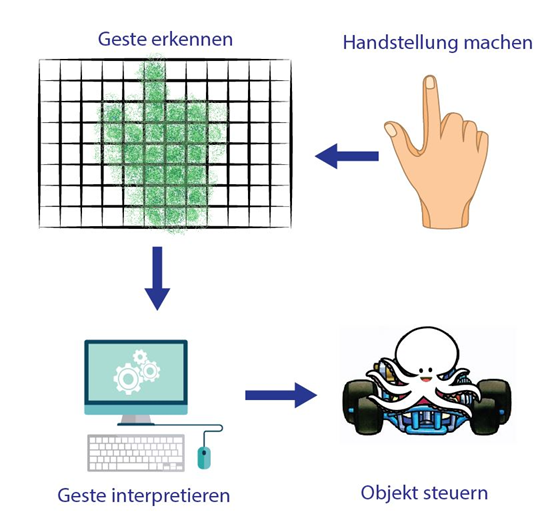
\includegraphics[scale=1.3]{../figures/AblaufGestikulaser.png}
	\caption{Schematischer Darstellung der Funktionsweise des Gestikulasers.}
	\label{fig:FunktionsweiseGestikulaser}
\end{figure}

\section{Die Beta-Version}
Während der Konstruktion unseres Gestikulasers erstellten wir eine vorläufige Photoplatte, bei der die Photodioden in einem festgelegten Muster auf der Oberseite der einer Holzplatte angebracht waren. Damit war der erste Meilenstein geschafft: Unsere Idee funktionierte und wir konnten verschiedene Gesten erkennen.

\begin{figure}[h]
	\centering
	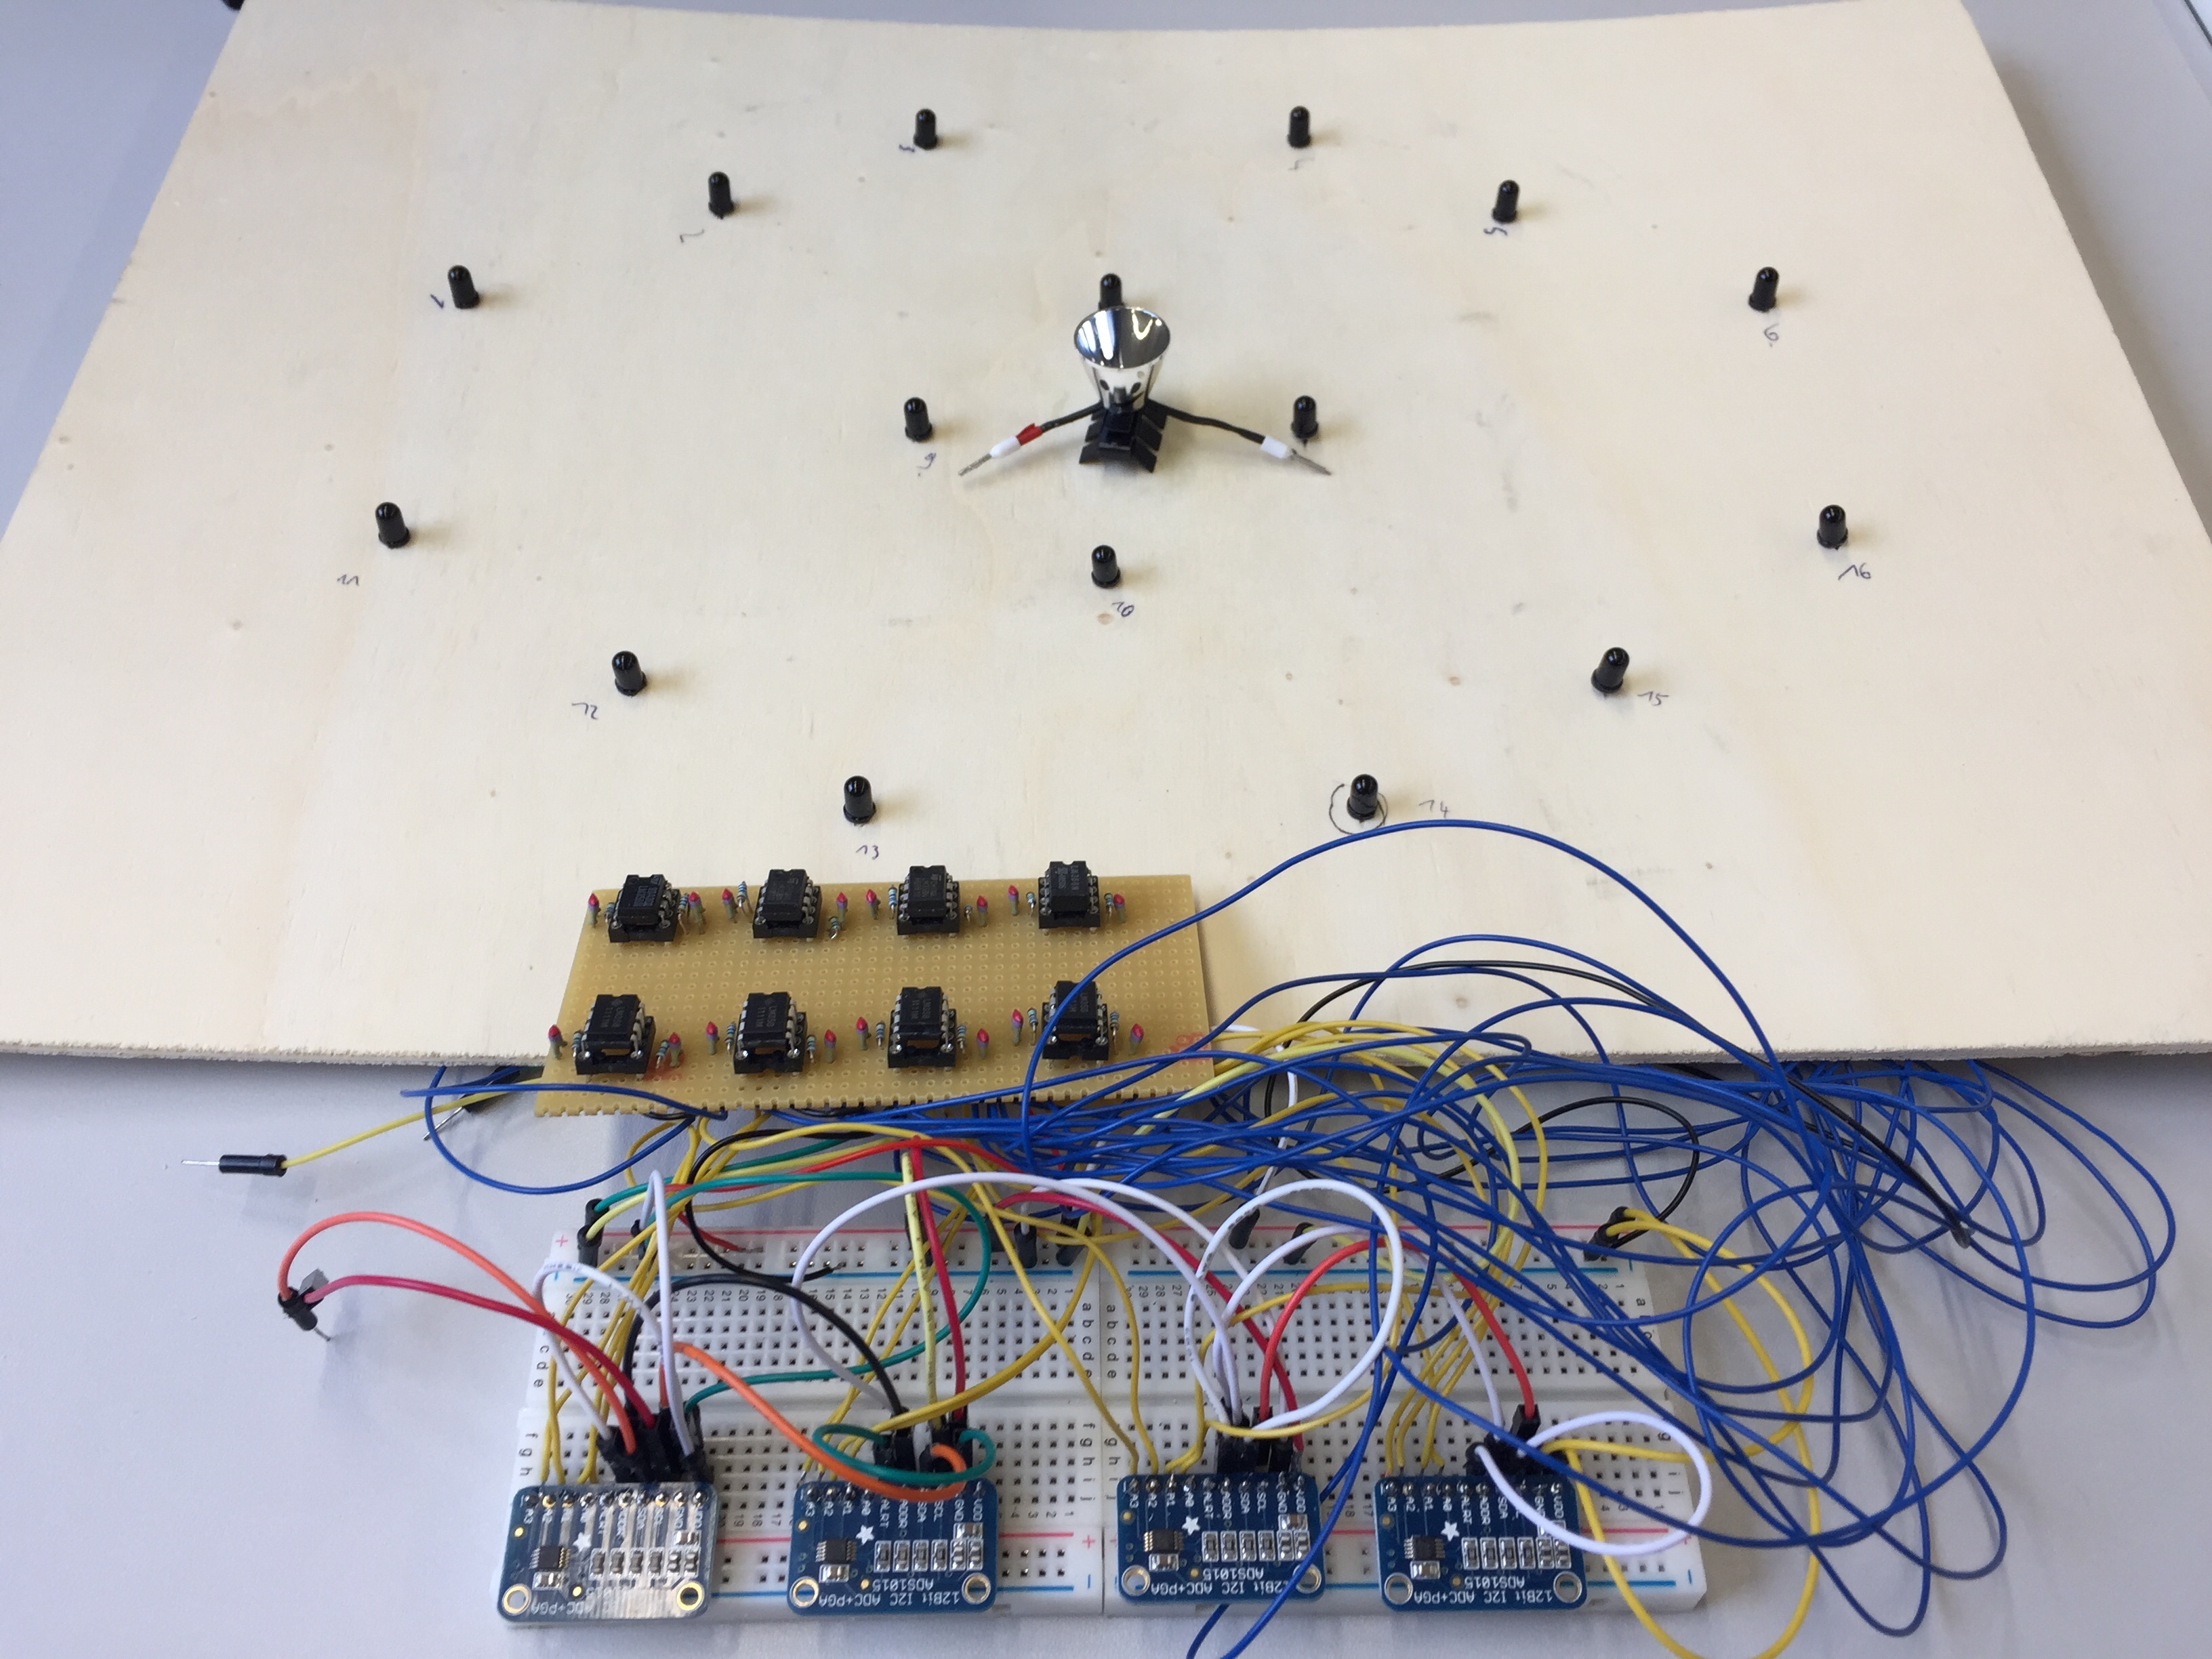
\includegraphics[scale=0.35]{../figures/PhotoplatteBeta.jpeg}
	\caption{Die Beta-Verion der Photoplatte: Ein Wust an Kabelsalat, dazu schwer zu transportieren und nicht modular!}
	\label{fig:PhotoplatteBeta}
\end{figure}

Nachdem unsere Idee funktionierte, wollten wir nun unseren Gestikulaser modularer zu gestalten. Eine aus verschiedenen Steckmodulen zusammensetzbare Photoplatte sollte nun helfen, dieses Ziel zu erreichen.

\section{Photoplatte}
Die neue Photoplatte besteht aus zwei verschiedenen Teilen, dem \textit{Oktokommander} als Herzstück der Photoplatte und passend dazu sieben \textit{Detektormodulen}. Die Detektormodule werden über USB-Anschlüsse an den Oktokommander angeschlossen. Der Microcontroller im Oktokommander wird mit einem zusätzlichen Datenkabel mit einem PC verbunden, auf dem die Software läuft.

\begin{figure}[h]
	\centering
	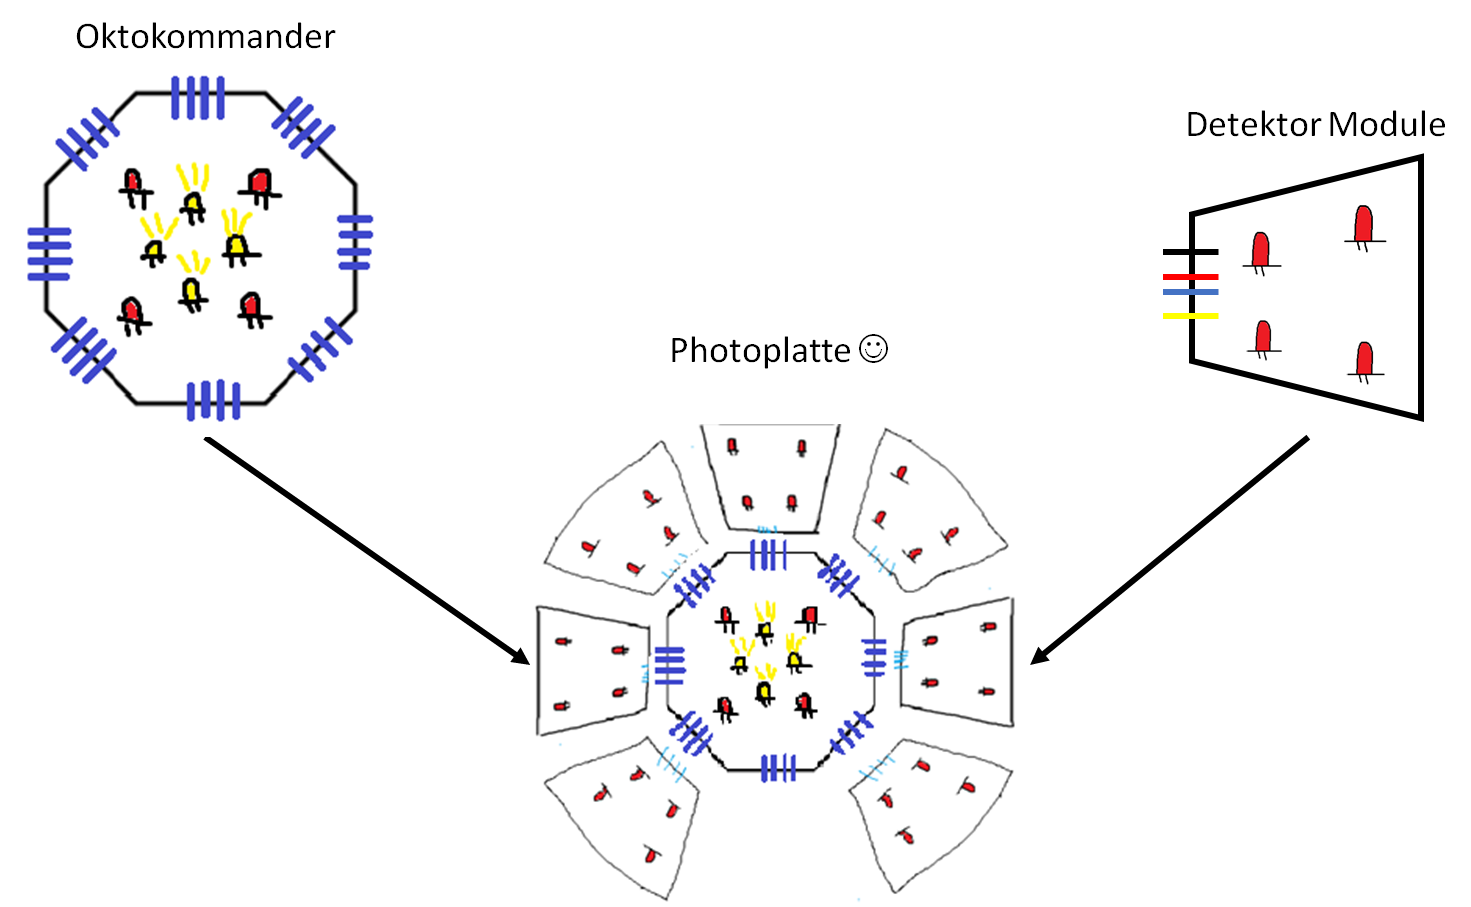
\includegraphics[scale=0.8]{../figures/Photoplatte.png}
	\caption{Die neue modulare Photoplatte setzt sich aus dem Oktokommander und den Detektormodulen zusammen.}
	\label{fig:PhotoplatteAlpha}
\end{figure}

\section{Oktokommander}
Der Oktokommander ist das Steuersystem der gesamten Photoplatte. Er besteht aus:
\begin{itemize}
	\item Einem Arduino Micro
	\item Einem i2c Expander
	\item Einem i2c Multiplexer inklusive Verstärkerschaltung
	\item Vier Photodioden
	\item Vier infrarot LED Quellen
	\item Sieben USB-Anschlüssen für die Detektormodule
\end{itemize}

\begin{figure}[h]
	\centering
	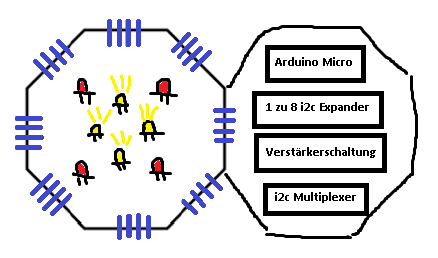
\includegraphics[scale=1.3]{../figures/OktokommanderOffen.png}
	\caption{Ein Blick auf die Innenteile des Oktokommanders.}
	\label{fig:Oktokommander}
\end{figure}

\section{Detektormodul}
Die Detektormodule enthalten jeweils 
\begin{itemize}
	\item vier Photodioden zur Detektion der Lichtreflexionen der Hand
	\item einen i2c Multiplexer inklusive Verstärkerschaltung
\end{itemize}
Sie werden über einen USB-Port an den Oktokommander angeschlossen. 

\begin{figure}[h]
	\centering
	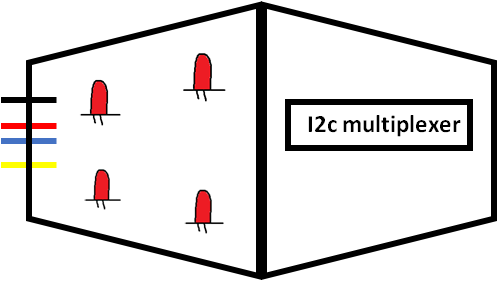
\includegraphics[scale=1.3]{../figures/DetektormodulOffen.png}
	\caption{Ein Blick auf die Innenteile eines Detektormoduls.}
	\label{fig:Detektormodul}
\end{figure}

\section{Software}
Für den Gestikulaser wurden zwei Software Komponenten entwickelt: In der Trainingsphase nimmt der Nutzer Messdaten der Photodioden von zuvor definierten Gesten auf. Mit Hilfe dieser Daten wird dann ein neuronales Netz trainiert, das es im Live-Betrieb ermöglicht, direkt aus den gemessenen Sensordaten die vom Nutzer gemachte Geste zu bestimmen. Bei der verwendeten Software wurden nur open-source verfügbare Programme und Bibliotheken eingesetzt: Die Kommunikation zwischen dem Mikrocontroller und dem Computer erfolgt über \texttt{Python} Skripte, für die Erstellung des neuronalen Netzes wurde \texttt{TensorFlow}\texttrademark verwendet.

\begin{figure}[h]
	\centering
	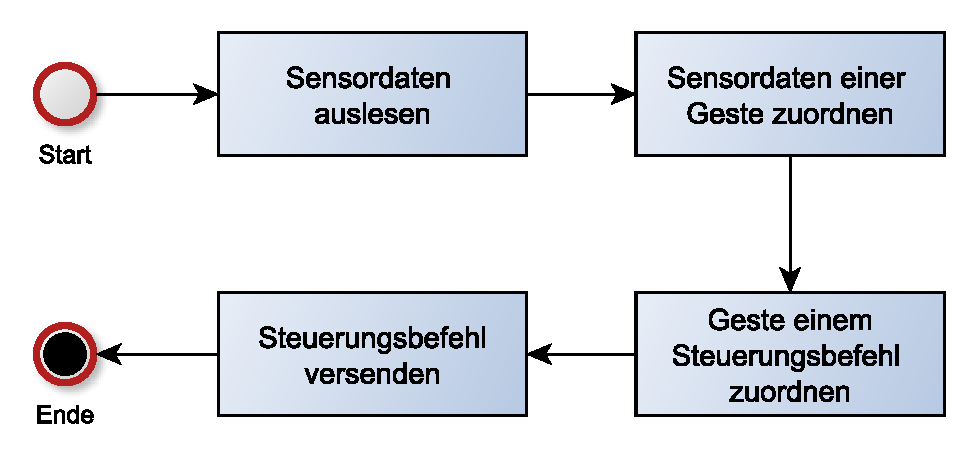
\includegraphics[scale=0.75]{../figures/AblaufSteuerung.pdf}
	\caption{Ablaufdiagramm der Software im Live-Betrieb.}
	\label{fig:AblaufSteuerung}
\end{figure}

\section{Ausblick}
Als Ausblick unseres Gestikulaser wäre eine Verfeinerung der aktuell durchführbaren Gestenerkennung denkbar, die nicht nur die Stellung der Hand, sondern auch die Krümmung der einzelnen Finger berücksichtigt. Zu diesem Zweck wurde bereits ein Prototyp für einen Sensorhandschuh entwickelt.

\begin{figure}[h]
	\centering
	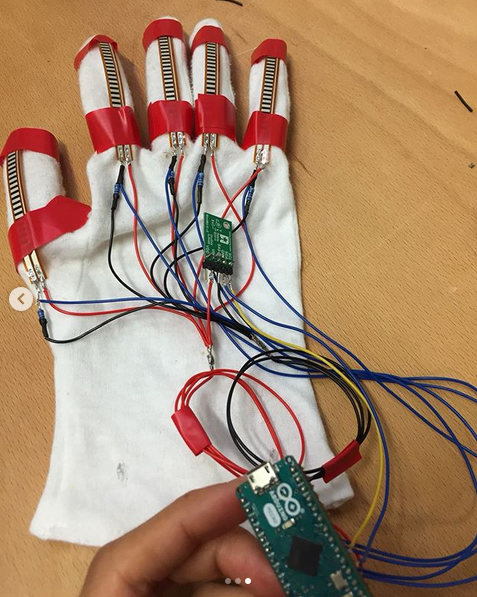
\includegraphics[scale=1.4]{../figures/Sensorhandschuh}
	\caption{Aktueller Prototyp des Sensorhandschuhs. Es sind Biegesensoren für alle Finger, ein Gyroskop und ein Beschleunigungssensor im Einsatz. Die Sensordaten 
	werden von einem Arduino Micro verarbeitet.}
	\label{fig:Sensorhandschuh}
\end{figure}

\section{Sponsoren}
Ein besonderen Dank gilt unseren Sponsoren: \\
\begin{tabularx}{\textwidth}{p{10cm} c}
	Aconity3D GmbH & \noindent\parbox[c]{\hsize}{
\includegraphics[scale=1]{../Logos/aconity.png}} \\
	& \\
	Fraunhofer ILT & \noindent\parbox[c]{\hsize}{
\includegraphics[scale=1.2]{../Logos/ILT.png}} \\
	& \\
	Würth Electronik GmbH \& Co. KG & \noindent\parbox[c]{\hsize}{
\includegraphics[scale=0.1]{../Logos/Wuerth.png}}
\end{tabularx} \\

\end{multicols}

\conference{
	\raisebox{0.5cm}[0cm]{
\includegraphics[height=3cm]{../Logos/VDE.png} } \hfill
	\raisebox{1.25cm}[0cm]{
\includegraphics[height=1.5cm]{../Logos/Faulhaber.png}} \hfill
	\raisebox{0cm}[0cm]{
\includegraphics[height=4cm]{../Logos/micronit.png}} \hfill
	\raisebox{0cm}[0cm]{
\includegraphics[height=4cm]{../Logos/electronica.png}} \hfill 
	\raisebox{0cm}[0cm]{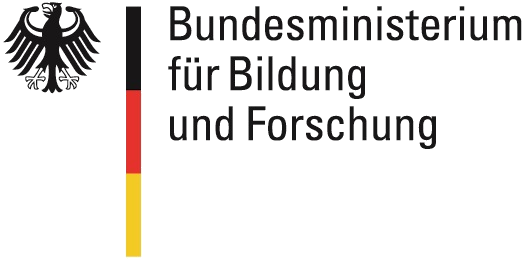
\includegraphics[height=4cm]{../Logos/BMBF.png}}
}

\end{document}